\documentclass[border=10pt]{standalone}
\usepackage{tikz}
\usetikzlibrary{calc}
\begin{document}
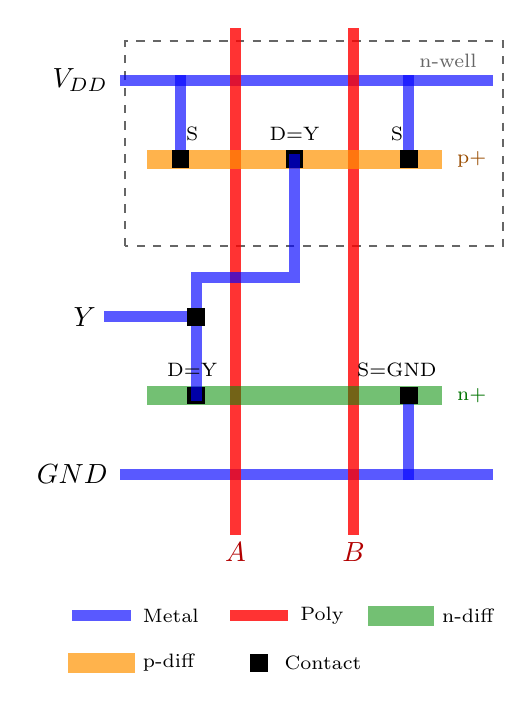
\begin{tikzpicture}[scale=1.0,
  metal/.style={blue, line width=4pt, line cap=rect, opacity=0.65},
  poly/.style={red, line width=4pt, line cap=rect, opacity=0.8},
  ndiff/.style={green!55!black, line width=7pt, line cap=rect, opacity=0.55},
  pdiff/.style={orange!85!yellow, line width=7pt, line cap=rect, opacity=0.7},
  contact/.style={draw=black, fill=black, minimum size=6pt, inner sep=0pt},
  nwell/.style={dashed, draw=black!60, line width=0.8pt}]

  % n-well around PMOS region
  \draw[nwell] (0.6,2.9) rectangle (5.4,5.5);
  \node[black!60] at (4.7,5.25) {\scriptsize n-well};

  % VDD / GND metal rails
  \draw[metal] (0.6,5) -- (5.2,5);  \node[left] at (0.5,5){$V_{DD}$};
  \draw[metal] (0.6,0) -- (5.2,0);  \node[left] at (0.5,0){$GND$};

  % polysilicon gates A and B (vertical, cross both diffusions)
  \draw[poly] (2.0,-0.7) -- (2.0,5.6);  \node[red!70!black,below] at (2.0,-0.75){$A$};
  \draw[poly] (3.5,-0.7) -- (3.5,5.6);  \node[red!70!black,below] at (3.5,-0.75){$B$};

  % p-diffusion (the two PMOS share it): [S|gA|D|gB|S]
  \draw[pdiff] (1.0,4) -- (4.5,4);  \node[orange!60!black] at (5.0,4){\scriptsize p+};
  % n-diffusion (the two NMOS share it): [D|gA|mid|gB|S]
  \draw[ndiff] (1.0,1) -- (4.5,1);  \node[green!45!black] at (5.0,1){\scriptsize n+};

  % PMOS sources -> VDD (left & right ends of p-diff)
  \draw[metal] (1.3,5)--(1.3,4);  \node[contact] at (1.3,4){};
  \draw[metal] (4.2,5)--(4.2,4);  \node[contact] at (4.2,4){};
  % NMOS source -> GND (right end of n-diff)
  \draw[metal] (4.2,0)--(4.2,1);  \node[contact] at (4.2,1){};

  % output Y : p-diff drain (middle) tied to n-diff drain (left end)
  \node[contact] at (2.75,4){};        % PMOS drain contact
  \node[contact] at (1.5,1){};         % NMOS drain contact
  \draw[metal] (2.75,4) -- (2.75,2.5) -- (1.5,2.5) -- (1.5,1);
  \draw[metal] (1.5,2.0) -- (0.4,2.0); \node[contact] at (1.5,2.0){};
  \node[left] at (0.35,2.0) {$Y$};

  % helper labels for regions
  \node[black] at (1.45,4.32){\scriptsize S}; \node[black] at (2.75,4.32){\scriptsize D=Y};
  \node[black] at (4.05,4.32){\scriptsize S};
  \node[black] at (1.45,1.32){\scriptsize D=Y}; \node[black] at (4.05,1.32){\scriptsize S=GND};

  % ---- legend ----
  \begin{scope}[shift={(0,-2.3)}]
    \draw[metal]  (0,0.5)--(0.6,0.5); \node[right] at (0.7,0.5){\scriptsize Metal};
    \draw[poly]   (2.0,0.5)--(2.6,0.5); \node[right] at (2.7,0.5){\scriptsize Poly};
    \draw[ndiff]  (3.8,0.5)--(4.4,0.5); \node[right] at (4.5,0.5){\scriptsize n-diff};
    \draw[pdiff]  (0,-0.1)--(0.6,-0.1); \node[right] at (0.7,-0.1){\scriptsize p-diff};
    \node[contact] at (2.3,-0.1){}; \node[right] at (2.5,-0.1){\scriptsize Contact};
  \end{scope}
\end{tikzpicture}
\end{document}
